% ============================================================
%  The Climate Standoff — Dissertation
%  Compile: pdflatex dissertation.tex  (run twice for refs)
%  Assets resolved via \graphicspath from latex/ directory
% ============================================================
\documentclass[10pt,a4paper]{article}

\usepackage[margin=2.5cm]{geometry}
\usepackage{graphicx}
\usepackage{booktabs}
\usepackage{amsmath,amssymb}
\usepackage{setspace}
\usepackage[hidelinks]{hyperref}
\usepackage{parskip}
\usepackage{microtype}
\usepackage{enumitem}
\usepackage{float}
\usepackage{placeins}  % \FloatBarrier
\usepackage{needspace}
\usepackage{caption}
\captionsetup[figure]{labelformat=empty}
\usepackage{tikz}
\usetikzlibrary{arrows.meta, positioning, calc}
\usepackage{pgfplots}
\pgfplotsset{compat=1.18}

\graphicspath{
  {../results/dissertation/}
  {../results/figures/}
}

\setstretch{1.4}
\setlength{\parindent}{0pt}
\setlength{\parskip}{0.8em}

\widowpenalty=10000
\clubpenalty=10000
\displaywidowpenalty=10000
\interlinepenalty=500

% ── Title helpers ─────────────────────────────────────────
\newcommand{\disssubtitle}[1]{\textit{\Large #1}}
\newcommand{\bpar}[1]{\medskip\noindent\textbf{#1}\par}

% ── Convenience: bloc colours not needed in text ──────────
\begin{document}

% ============================================================
%  TITLE PAGE
% ============================================================
\begin{titlepage}
\vspace*{0.4cm}
{\noindent\LARGE\textbf{The Climate Standoff:}\\[0.3em]
\large\textit{A Dynamic Game Model of Strategic Tipping in Global Climate Coordination}
\par}

\vspace{0.8cm}

\textbf{Abstract}

\medskip
This paper develops a finite-horizon dynamic Markov game of global climate coordination among four
heterogeneous blocs: the United States, China, the European Union, and a Rest of World aggregate
comprising large emerging economies (Brazil, India, Mexico, Vietnam, and their peers) at
intermediate stages of industrial development. Each period, blocs choose whether to adopt a low-carbon
transition; adoption is irreversible. Transition costs fall endogenously through learning spillovers, political
pressure rises with coalition size, and collective benefits accrue once a weighted participation threshold is
crossed. Behaviour is characterised using quantal response equilibrium (QRE), which replaces the
knife-edge solutions of Nash-based coalition models with smooth probabilistic choice, permitting
well-behaved comparative statics across the full parameter space. Cardinal payoff weights are recovered by
Simulated Method of Moments, anchoring the model to the 2025 strategic environment.

We conduct two experiments: marginal parameter sweeps that identify how far each lever must move to compress coordination failure, and global sensitivity analysis that jointly perturbs the full parameter space across 1,000 draws to test whether those rankings survive simultaneous variation. Both are complemented by functional-form robustness checks.

We find that jointly extending the effective planning horizons of the United States and China is the most
powerful single intervention: it is the only lever that drives coordination success to near-certainty under a
modest bilateral improvement. China's domestic transition cost burden is an independent bottleneck that
longer horizons alone cannot resolve; targeted cost reduction through technology transfer or concessional
finance is a necessary complement. Perceived feasibility is itself a coordination determinant: institutions
that make partial progress visible accelerate adoption without altering underlying incentives.

We document a novel asymmetry in rationality spillovers. Reducing volatility in US climate policy improves
coordination outcomes both directly and by disciplining Chinese strategic expectations; mediation analysis
attributes 86 per cent of the $\lambda_{US}$ effect on coordination timing to this expectations channel.
Greater Chinese policy coherence does not generate a reciprocal effect on US expectations.

\vfill
\noindent\textbf{Author:} David Clements\\
\textbf{Supervisor:} Todd R.\ Kaplan\\
\textbf{Academic Year:} 2026\\
\textbf{Word Count:} 9,786
\end{titlepage}

\clearpage
\tableofcontents
\clearpage

% ============================================================
%  1.  INTRODUCTION
% ============================================================
\clearpage
\needspace{12em}
\section{Introduction}

Threshold public goods models explain coordination failure through two interlocking mechanisms:
collective benefits depend on reaching a critical participation mass, and multiple equilibria make that
mass difficult to attain. The literature has produced elegant characterisations of why cooperation stalls. It
has been less successful at explaining why it sometimes accelerates.

The most consequential recent shifts in climate policy were not preceded by formal treaties. The EU's Carbon Border Adjustment Mechanism became politically viable only after domestic decarbonisation created the incentive to export climate standards through trade policy. The US Inflation Reduction Act reshaped global clean-energy investment through large-scale subsidies, triggering competitive policy responses across Europe and Asia within eighteen months. In both cases, early movers altered the payoff matrix for everyone else; the institutional architecture followed strategic logic rather than producing it.

The strategic environment is a multilateral game of chicken among highly asymmetric players. A small number are systemically important enough that their inaction carries disproportionate global consequences, placing them under asymmetric pressure to move first. Others face weak early-mover incentives because short political horizons and high transition costs raise the price of unilateral action. Still others face greater climate vulnerability and less room to wait. The coordination problem is shaped not only by whether blocs eventually cooperate, but by who can afford to delay and whose move most strongly updates others' incentives.

Standard treaty-based models abstract from these features. By treating enforcement pressure, cost trajectories, and threshold progress as exogenous, they cannot account for the timing, escalation, and asymmetry that define modern climate geopolitics.


% ============================================================
%  2.  REVIEW OF LITERATURE
% ============================================================
\clearpage
\needspace{12em}
\section{Review of Literature}

\needspace{12em}
\subsection*{Equilibrium Concepts: Nash to Quantal Response}

The dominant solution concepts in the climate cooperation literature share a common assumption: players
best-respond exactly to the strategies of others. Barrett (1994) uses stage-game Nash equilibrium and
renegotiation-proof repeated-game equilibrium to characterise self-enforcing international environmental
agreements. Harstad (2016) selects Markov perfect equilibrium on the grounds that strategies depending
only on payoff-relevant state variables are both analytically tractable and behaviourally plausible. The
assumption of exact best response is not incidental to these frameworks. It is load-bearing.

Carraro and Siniscalco (1993) establish the classical fragility result: stable coalitions under internal and
external stability conditions are typically small, and because participation decisions are discrete, small
parameter changes induce large discontinuous shifts in equilibrium coalition size. The framework moves
abruptly between near-full cooperation and near-complete defection, which limits its usefulness precisely
where the empirical record is most interesting: the margin where marginal incentive changes produce
cascading adoption rather than stasis.

Quantal response equilibrium resolves this by replacing exact best response with probabilistic choice
(McKelvey and Palfrey, 1995). Players choose better options more often, but not always, with choice
probabilities increasing in expected payoffs governed by the rationality parameter $\lambda$. A marginal increase
in adoption costs therefore reduces adoption probability incrementally rather than flipping participation
off entirely. Goeree, Holt, and Palfrey (2003) show that QRE closely tracks observed behaviour across a
wide range of laboratory strategic environments.

The calibrated value of $\lambda$ carries direct substantive content. Putnam (1988) formalises why governments
cannot behave as frictionless unitary optimisers: international commitments must remain feasible in the
domestic ratification game. In this setting, stochastic choice is a reduced-form representation of those
political frictions rather than purely behavioural error. The noise in $\lambda$ reflects domestic win sets,
bureaucratic friction, and electoral uncertainty, not irrationality.

Practical uniqueness is confirmed by convergence to identical fixed points across multiple initialisations; full convergence diagnostics are in the appendix.

QRE ensures smooth incentive changes produce smooth behavioural responses. It does not explain when those responses accumulate into self-reinforcing adoption cascades.

\needspace{12em}
\subsection*{Strategic Tipping and Diffusion Dynamics}

The physical and technological foundations of tipping are reasonably well understood. Way et al.\ (2022)
show that endogenous cost declines through fast learning curves for renewables can shift mitigation
pathways more sharply than most integrated assessment models assume, a finding consistent with the
directed technical change literature establishing that innovation incentives respond to deployment scale in
ways that can generate self-reinforcing cost trajectories (Acemoglu et al., 2012). Farmer et al.\ (2019)
introduce sensitive intervention points in socioeconomic systems, arguing that small, well-targeted
interventions can exploit these amplification mechanisms to trigger cascading low-carbon transitions.
Otto et al.\ (2020) identify specific social subsystems where positive feedback could rapidly compress
emissions trajectories, and Sharpe and Lenton (2021) extend this into a framework of upward-scaling
tipping cascades in which activating one socio-technical tipping point raises the probability of triggering
the next. Milkoreit et al.\ (2018) formalise the social tipping point concept across interdisciplinary
contexts, identifying belief shifts and perceived feasibility as distinct triggers alongside cost and
technology channels.

These contributions capture dynamics observed in real energy transitions. They share a structural
limitation. Adoption decisions are embedded in aggregate diffusion mechanisms, systems feedback
frameworks, or reduced-form cost trajectories rather than arising from explicit strategic interaction
between heterogeneous countries. This matters because the mechanism is difficult to identify. Comin and
Hobijn (2010) document precisely this puzzle in a long historical panel of technology diffusions:
structurally similar countries adopt at systematically different speeds, with institutional and political
factors explaining residual variation that cost differentials alone cannot. Without an explicit strategic
foundation, it is difficult to distinguish whether cascades emerge from cost feedbacks, expectation shifts,
or politically mediated peer effects; the policy implications of each differ sharply.

A second problem compounds the first. Tipping behaviour in formally specified models is often sensitive
to chosen parameter values, making it difficult to distinguish structurally robust dynamics from
calibration artefacts. A finding that holds only at a particular cost trajectory or rationality parameter is not
a finding about tipping. It is a finding about one point in the parameter space.

Taken together, these gaps motivate a framework that endogenises tipping through asymmetric strategic interaction, with a disciplined method for establishing which dynamics survive joint parameter perturbation.

\needspace{12em}
\subsection*{Gaps and Contribution}

Two gaps run through the literature reviewed above. The first is structural. Existing frameworks rarely
model declining costs, endogenous political pressure, and asymmetric influence as joint strategic
determinants of cooperation. Agreement-based models treat enforcement as exogenous: Barrett (1994)
characterises self-enforcing agreements under fixed participation incentives, and Nordhaus (2015)
demonstrates that coalition models generate stable but small cooperative groups precisely because the
strategic environment outside the coalition is held constant. Diffusion models embed adoption in
aggregate cost functions or reduced-form trajectories rather than strategic interaction (Grubb et al., 2021).
Neither tradition explains how early adoption by anchor players reshapes the incentives of holdouts over time.

The second gap is methodological. Kolstad (2007) documents that quantitative results in the IEA literature shift substantially across plausible cost and benefit assumptions, yet few studies distinguish the cross-bloc structure pinned down by observable data from the latent cardinal strength of the payoff channels. Most approaches calibrate to a single benchmark or rely on ad hoc sensitivity checks, making it difficult to tell whether a finding reflects a structural property of the game or a feature of one point in the parameter space.

This paper addresses both gaps. A finite-horizon Markov game with heterogeneous blocs and irreversible adoption characterises behaviour using QRE, allowing smooth comparative statics without the brittleness of Nash-based coalition models.

Calibration is separated into two layers. The ordinal layer is identified from macroeconomic and emissions data. The cardinal layer is recovered by simulated method of moments (McFadden, 1989), matching observable features of the contemporary climate transition: EU leadership, strategic free-riding by major emerging economies, and the delayed onset of self-reinforcing adoption. These produce a single fitted baseline anchored to the 2025 strategic environment.

Marginal sweeps identify which channels matter in isolation. Global sensitivity analysis (Saltelli et al., 2008) stress-tests the rankings by jointly perturbing the full parameter space, separating levers that are locally powerful from those that remain influential once the wider strategic environment moves.

% ============================================================
%  3.  MODEL
% ============================================================
\clearpage
\needspace{12em}
\section{Model}

\needspace{12em}
\subsection*{Players and Structure}

\[
i \in \{\text{US, EU, CN, RoW}\}
\]

Each player represents a geopolitical bloc with distinct economic structures, emissions profiles,
and strategic incentives. Using representative blocs rather than individual countries is standard
in the climate cooperation literature and preserves the asymmetries that shape global outcomes
while maintaining tractability. The United States, European Union, and China together dominate
global emissions, renewable manufacturing capacity, and geopolitical influence. The Rest of
the World aggregates developing and emerging economies whose individual influence is limited
but whose collective climate vulnerability is high. This structure captures a central asymmetry
of the cooperation problem: the blocs with greatest capacity to drive coordination often face
weaker direct climate incentives, while those with the strongest incentives face limited individual
leverage.

\begin{figure}[htbp]
\centering
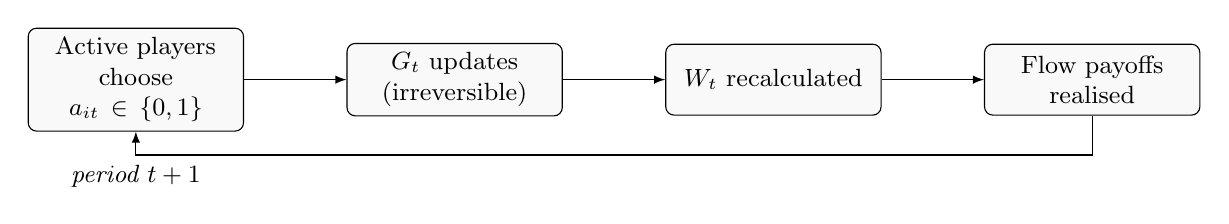
\begin{tikzpicture}[>=latex, node distance=0.5cm and 1.3cm,
  box/.style={draw, rounded corners=3pt, text width=2.5cm, align=center,
              minimum height=0.9cm, font=\small, fill=gray!5}]
\node[box] (a) {Active players\\ choose $a_{it} \in \{0,1\}$};
\node[box, right=of a] (b) {$G_t$ updates\\ (irreversible)};
\node[box, right=of b] (c) {$W_t$ recalculated};
\node[box, right=of c] (d) {Flow payoffs\\ realised};
\draw[->] (a) -- (b);
\draw[->] (b) -- (c);
\draw[->] (c) -- (d);
\draw[->] (d.south) -- ++(0,-0.5) -| node[below, midway, font=\small\itshape]{period $t+1$} (a.south);
\end{tikzpicture}
\caption{Game flow diagram. Each period, active players simultaneously choose whether to adopt.
The adoption vector updates, weighted coalition mass $W_t$ is recalculated, and flow payoffs
are realised before the game advances to the next period.}
\label{fig:game_flow}
\end{figure}

Time is discrete and finite, indexed by $t = 1, 2, \ldots, T$, where each period represents
five years. The finite horizon is not a technical convenience. $T$ represents the point beyond which cumulative emissions lock in irreversible physical damages: tipping elements in the climate system, ice-sheet dynamics, and permafrost feedbacks impose a hard deadline on collective action, consistent with IPCC AR6 and Lenton et al.\ (2019) on biophysical tipping points beyond which further mitigation cannot restore the prior climate state. Beyond $T$ the coordination problem closes rather than continuing in a weakened form. Each period of delay compounds irreversibly, and the value of early coordination derives from the window's closure. In each period, active
players simultaneously choose a current-period action $a_{it} \in \{0, 1\}$, where $a_{it} = 1$
denotes adoption. Cumulative adoption status evolves according to the stock-flow law of motion:
\[
G_{i,t+1} = G_{it} + (1 - G_{it})\, a_{it}, \qquad G_{i1} = 0
\]
This makes irreversibility explicit: once $G_{it} = 1$, the term $(1 - G_{it})$ zeroes out any
further action, so the player's status is locked regardless of $a_{it}$. The set of active
players in period $t$ is:
\[
\mathcal{A}_t = \{i : G_{it} = 0\}
\]
Only players in $\mathcal{A}_t$ face a non-trivial adoption decision. Already-adopted players
contribute nothing new to the state.

\begin{figure}[htbp]
\centering
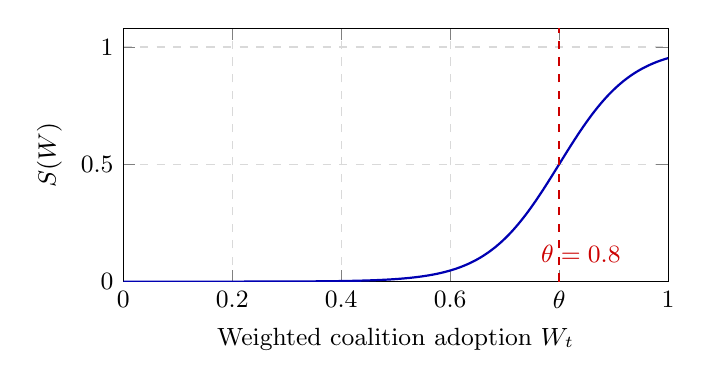
\begin{tikzpicture}
\begin{axis}[
  width=8.5cm, height=4.8cm,
  xlabel={Weighted coalition adoption $W_t$},
  ylabel={$S(W)$},
  xmin=0, xmax=1, ymin=0, ymax=1.08,
  xtick={0,0.2,0.4,0.6,0.8,1.0},
  xticklabels={$0$,$0.2$,$0.4$,$0.6$,$\theta$,$1$},
  ytick={0,0.5,1},
  grid=major, grid style={dashed,gray!30},
  tick label style={font=\small},
  label style={font=\small},
]
\addplot[thick, blue!70!black, domain=0:1, samples=200]
  {1/(1+exp(-15*(x-0.8)))};
\addplot[dashed, red!80!black, thick] coordinates {(0.8,0)(0.8,1.08)};
\node[font=\small, text=red!80!black] at (axis cs:0.84,0.12) {$\theta=0.8$};
\end{axis}
\end{tikzpicture}
\caption{State visualisation. The sigmoid $S(W)$ shows how the stabilisation benefit
activates as cumulative weighted adoption crosses the coordination threshold $\theta = 0.8$.
Benefits concentrate sharply around $\theta$ under the baseline steepness $\eta = 15$;
the dashed line marks where collective action tips from partial to near-full coordination relief.}
\label{fig:state_viz}
\end{figure}

Each player $i$ is assigned an influence weight $w_i > 0$, normalised so that $\sum_i w_i = 1$.
Influence asymmetry is central to the model's tipping dynamics: early adoption by the US or
China can shift the aggregate state substantially in a single period, while equivalent action
by smaller players cannot.

The payoff-relevant state is the full adoption vector together with elapsed time:
\[
s_t = (t, G_t), \qquad G_t = (G_{1t}, G_{2t}, G_{3t}, G_{4t})
\]
Because costs $c_i(\cdot)$, damages $d_i(\cdot)$, and pressure $p_i$ are player-specific,
the identity of who has adopted matters for future incentives: two configurations generating
the same weighted total $W_t$ can imply different active sets and different continuation values.
Cumulative weighted adoption:
\[
W_t \equiv \sum_i w_i G_{it}
\]
is a derived statistic used throughout the payoff functions. Strategies are written as functions
of $(t, W_t)$ for notational clarity where context permits, but the backward induction algorithm
tracks the full adoption vector $G_t$ to correctly compute transition probabilities and identify
active players at each node.

\subsubsection*{Irreversibility of Adoption}

Adoption is modelled as irreversible: once $G_{it} = 1$, the state is locked for all subsequent
periods. This is a simplifying assumption, but one grounded in the economics of large-scale
energy transition. Grid infrastructure, renewable capacity, and retooled industrial supply chains
represent substantial sunk investments whose abandonment would impose severe economic losses.
A government that has restructured its energy system around renewable capacity cannot cheaply
reinstate fossil fuel infrastructure even if political conditions change.

Full irreversibility is the limiting case of a costly reversal environment. Perfect reversibility would generate a degenerate outcome: blocs could adopt, observe whether the coalition reaches the threshold, and costlessly undo their commitment. The assumption preserves the genuine commitment risk at the heart of the model.

\begin{figure}[htbp]
\centering
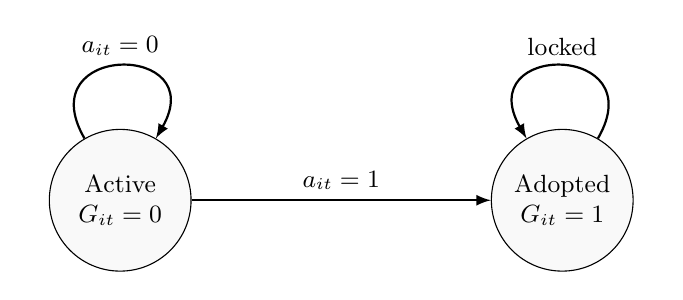
\begin{tikzpicture}[>=latex, node distance=3.8cm,
  st/.style={draw, circle, minimum size=1.8cm, align=center, font=\small, fill=gray!5}]
\node[st] (active) {Active\\ $G_{it}=0$};
\node[st, right=of active] (locked) {Adopted\\ $G_{it}=1$};
\draw[->, thick] (active) -- node[above, font=\small]{$a_{it}=1$} (locked);
\draw[->, thick] (active) to[out=120,in=60,looseness=4]
  node[above, font=\small]{$a_{it}=0$} (active);
\draw[->, thick] (locked) to[out=60,in=120,looseness=4]
  node[above, font=\small]{locked} (locked);
\end{tikzpicture}
\caption{Lock-in and lock-out dynamics. Once a bloc adopts ($G_{it}=1$), its state is
permanently locked. Early movers cannot defect, while holdouts face an escalating cost of
delay as the coalition grows.}
\label{fig:lockin}
\end{figure}

\needspace{12em}
\subsection*{Coordination Threshold and Stabilisation}

Collective benefits are non-linear in participation. Rather than a hard threshold where
stabilisation switches on instantaneously, benefits are governed by a smooth sigmoid centred
at $\theta$:
\[
S(W) = \frac{1}{1 + \exp(-\eta(W - \theta))}
\]
where $\eta > 0$ controls the steepness of the transition. Partial coordination delivers partial
benefit, consistent with climate science evidence that incremental mitigation reduces damages
even absent full stabilisation. Marginal returns to coordination are highest near $\theta$,
generating the threshold dynamics central to the model. As $\eta \to \infty$, $S(W)$ approaches
a step function at $\theta$, so the hard threshold case is a limiting special case rather than a
separate model. Both $\theta$ and $\eta$ are varied in the sensitivity analysis.

This threshold structure generates the model's core strategic tension. Early adoption imposes immediate transition costs but delivers negligible benefit: $S(W)$ is flat well below $\theta$, so a lone early mover shifts their own cost burden without materially accelerating stabilisation. The collective benefit only becomes substantial as the coalition approaches critical mass. Patience, attainability beliefs, and the composition of the early coalition are therefore the dominant strategic variables.

\needspace{12em}
\subsection*{Flow Payoffs}

All flow payoffs in period $t$ are evaluated at $W_t$, the cumulative adoption state at the
\textit{start} of the period, before current actions are realised. Under simultaneous choice,
no player observes others' period-$t$ decisions when choosing. Adopters incur the one-off
transition cost in the period of adoption; any learning spillover from their own action enters
only future periods via $W_{t+1}$.

\bpar{Transition Costs:}
Adoption involves a one-off cost, paid only in the period of adoption, that declines with
cumulative adoption:
\[
c_i(W_t) = c_i^0 \left(1 - \gamma W_t\right)
\]
The parameter $c_i^0$ captures each bloc's baseline transition burden. The learning parameter
$\gamma \in [0,1]$ governs how quickly costs fall as adoption spreads, capturing technology
spillovers, supply chain deepening, and learning-by-doing.

\bpar{Climate Damages:}
Countries face damages that escalate over time and diminish as coordination approaches the
threshold:
\[
d_i(t, W_t) = d_i^0 \cdot (1 + \kappa t) \cdot (1 - S(W_t))
\]
The baseline vulnerability $d_i^0$ captures structural economic exposure to climate risk. The
temporal escalation term $(1 + \kappa t)$ introduces a deadline effect: the longer coordination
takes, the worse the consequences. Damages are non-excludable: only the collective level of
adoption $W_t$ matters, not any individual player's action.

\bpar{Political Pressure:}
Active players who delay face political pressure growing with coalition size. For $i \in
\mathcal{A}_t$:
\[
p_i \cdot W_t
\]
The pressure sensitivity $p_i$ reflects each bloc's exposure to trade restrictions, diplomatic
isolation, and reputational costs. The linear specification implies that holding out becomes
proportionally more costly as the coalition grows.

\bpar{Stabilisation Benefit:}
All players receive a per-period benefit as adoption approaches the threshold:
\[
b \cdot S(W_t)
\]
The benefit is non-excludable: even players who have not adopted receive it as the world
stabilises, preserving the free-rider incentive throughout the game.

\bpar{Combined Flow Payoffs:}
The state-contingent component received by all players regardless of action:
\[
r_i(t, W_t) = -d_i(t, W_t) + b \cdot S(W_t)
\]
For active players ($i \in \mathcal{A}_t$), the action-specific payoffs are:
\begin{align*}
r_i^A(t, W_t) &= -c_i(W_t) + r_i(t, W_t) \\
r_i^D(t, W_t) &= -p_i W_t + r_i(t, W_t)
\end{align*}
For already-adopted players ($i \notin \mathcal{A}_t$), the transition cost has been paid in
full and their period payoff is simply $r_i(t, W_t)$.

\bpar{Discount Factors:}
Each player $i$ is assigned a discount factor $\delta_i \in (0,1)$. A payoff received in
period $t+1$ is worth $\delta_i$ times the same payoff in period $t$. Higher values reflect
greater patience: a bloc that values future payoffs highly has stronger incentives to invest
in early coordination. Bloc-specific values are discussed in the Calibration section.

These two parameters capture conceptually distinct sources of strategic inertia and should
not be conflated. $\delta_i$ governs the length of a bloc's effective planning horizon:
how far into the future its institutions credibly weight consequences. $\lambda$ governs the
precision of strategic choice around that horizon: the degree of political noise, bureaucratic
friction, and domestic constraint that prevents even a patient bloc from acting as a
frictionless optimiser. A bloc can have a long planning horizon but high political noise
(high $\delta$, low $\lambda$), or a short horizon executed with institutional precision
(low $\delta$, high $\lambda$). The two parameters do different things and are identified
through different variation in the analysis.

\needspace{12em}
\subsection*{Recursive Value Structure}

Players are forward-looking. Q-values capture the full value of each action as current flow
payoffs plus discounted expected continuation. For active players $i \in \mathcal{A}_t$:
\begin{align*}
Q_i^A(s_t) &= r_i^A(t, W_t) + \delta_i\, \mathbb{E}[V_i(s_{t+1}) \mid a_{it} = 1] \\
Q_i^D(s_t) &= r_i^D(t, W_t) + \delta_i\, \mathbb{E}[V_i(s_{t+1}) \mid a_{it} = 0]
\end{align*}
The conditioning on $a_{it}$ matters: player $i$'s own action shifts $W_{t+1}$ by $w_i$ if
they adopt, altering the distribution over future states and the expected continuation value
of each choice. Terminal condition: $V_i(T+1, \cdot) = 0$.

For active players, the continuation value takes the log-sum-exp form:
\[
V_i(s_t) = \frac{1}{\lambda} \log\!\left(e^{\lambda Q_i^A} + e^{\lambda Q_i^D}\right)
\]
This is consistent with the assumption that players face i.i.d.\ Type~I Extreme Value payoff
shocks with scale $1/\lambda$. As $\lambda \to \infty$, $V_i(s_t) \to \max(Q_i^A, Q_i^D)$,
recovering the standard Bellman equation for a perfectly rational agent.

For already-adopted players ($i \notin \mathcal{A}_t$):
\[
V_i(s_t) = r_i(t, W_t) + \delta_i\, \mathbb{E}[V_i(s_{t+1})]
\]
Future utility continues to depend on the $W$ trajectory driven by the remaining active players.

\needspace{12em}
\subsection*{Equilibrium}

Equilibrium adoption probabilities are defined over active players and follow the logit QRE
formula. For $i \in \mathcal{A}_t$:
\[
\sigma_i(s_t) = \frac{\exp\{\lambda Q_i^A\}}{\exp\{\lambda Q_i^A\} + \exp\{\lambda Q_i^D\}}
\]
For $i \notin \mathcal{A}_t$, $\sigma_i(s_t) = 0$ by the irreversibility constraint.
Equilibrium is a fixed point in the mapping from beliefs over opponents' actions into optimal
logit response probabilities:
\[
\sigma^* = \mathrm{QRE}(Q(\sigma^*))
\]
No player wishes to revise their strategy given others' strategies, and others' strategies are
consistent with those beliefs. The game is solved by backward induction from period $T$. At
each state, fixed-point iteration finds the self-confirming probability vector.

\subsubsection*{Solution Method}

The finite horizon and irreversibility together make backward induction the natural and exact
solution method. The finite horizon provides a well-defined terminal condition $V_i(T+1,\cdot)=0$
from which the recursion unwinds cleanly. Irreversibility ensures the state space is
monotonically non-decreasing: once $G_{it}=1$, the player never returns to $\mathcal{A}_t$.
This bounds the number of distinct adoption configurations at each period to at most $2^4 = 16$,
making exhaustive enumeration computationally trivial. The backward induction algorithm stores
$\sigma_i(t, G_t)$ and $V_i(t, G_t)$ at each node, referenced by earlier periods without
recomputation. The full dynamic game is solved exactly in a single backward pass through the
game tree.

\needspace{12em}
\subsection*{State Transitions}

The adoption vector evolves according to:
\[
G_{i,t+1} = G_{it} + (1 - G_{it})\, a_{it} \qquad \forall\, i
\]
from which cumulative weighted adoption is derived:
\[
W_{t+1} = \sum_i w_i\, G_{i,t+1}
\]
For a given action profile $(a_{jt})_{j \in \mathcal{A}_t}$, the probability of moving from
$G_t$ to $G_{t+1}$ is:
\[
\Pr(G_{t+1} \mid G_t, \sigma) =
  \prod_{j \in \mathcal{A}_t} \sigma_j(s_t)^{a_{jt}} \left(1 - \sigma_j(s_t)\right)^{1-a_{jt}}
\]
Each active player's decision enters as an independent Bernoulli trial. Expected continuation
values sum over all reachable $G_{t+1}$:
\[
\mathbb{E}[V_i(s_{t+1}) \mid a_{it}] =
  \sum_{G_{t+1}} \Pr(G_{t+1} \mid G_t, \sigma, a_{it}) \cdot V_i(t+1, G_{t+1})
\]

% ============================================================
%  4.  CALIBRATION
% ============================================================
\clearpage
\needspace{12em}
\section{Calibration}

Implementing the model requires assigning numerical values to all parameters. Some can be disciplined
directly by observable data. Others cannot. The calibration strategy addresses this by separating the
problem into two layers, each with a distinct identification logic.

The first layer fixes ordinal structure: the relative positioning of blocs within each parameter channel. Cross-bloc rankings in transition costs, climate damages, and systemic influence can be inferred from data. The EU's position is identified from carbon intensity, trade openness, and deployment history; the SMM moments then target the magnitude of the EU--peer gap, not its existence. World Bank (2026) development indicators, national emissions inventories, and bilateral trade statistics provide the evidence base. This layer is held fixed throughout: perturbing it would mean contradicting the observable record.

The second layer recovers cardinal scaling: the relative importance governments place on transition costs, climate damages, and political pressure is not observable from macroeconomic data (Nordhaus, 2007) and is estimated using simulated method of moments (McFadden, 1989).

The moments represent the observable strategic fingerprint of the 2025 climate environment, each providing identifying variation for a specific payoff channel. The EU--US adoption gap and China's near-zero period-one probability identify the cost channel: a model with low $\alpha_c$ cannot reproduce early EU movement alongside near-zero Chinese activity. The EU leadership ratio identifies the benefit channel, capturing by how much the EU leads relative to peers with similar pressure exposure. Zero adoption by period two rules out parameterisations generating implausibly fast cascades. Mean coordination timing conditional on success anchors the speed at which the model tips once the coalition builds.

Ordinal structure is data-identified. Cardinal scaling is structurally estimated. The sensitivity analysis is conducted around this fitted baseline, which is what allows the distinction between locally powerful levers and structurally robust ones to carry empirical weight.

% ---- 4.1 Layer 1: Ordinal Structure -------------------------
\needspace{12em}
\subsection{Layer 1: Ordinal Structure}

\bpar{Per Player Params:}
Each per-player parameter is constructed from bloc-level data through a structural transformation
anchored to the EU as a reference bloc. This preserves empirical ordinal relationships across blocs while a
single scaling parameter alpha determines the absolute level.

\bpar{Transaction Costs:}
Transition costs are derived from the carbon intensity of GDP, constructed from World Bank (2026)
emissions and output data, adjusted for development. Carbon intensity captures the extent of structural
change required for decarbonisation: higher-intensity economies must replace more emissions-intensive
capital to meet the same mitigation target. Raw intensity cannot be taken at face value for less developed
economies, however. Low carbon intensity in those cases often reflects limited industrialisation rather
than genuinely clean infrastructure, which would falsely register as low transition costs.

To correct for this, a development-gated interpolation is applied. Each bloc's effective carbon intensity is
defined as a weighted average of its observed intensity and a global baseline, where the weight rises with
GDP per capita relative to the richest bloc, with all underlying series drawn from World Bank (2026)
national accounts and development indicators. Less developed economies are partially adjusted toward the
baseline, preventing the model from treating structural underdevelopment as a decarbonisation head start.

An affordability penalty is then applied on top. The cost of capital for renewable energy projects in
developing economies is empirically two to three times higher than in advanced economies, reflecting
financing constraints and weaker deployment capacity (Ameli et al., 2021). The affordability elasticity
(epsilon $\epsilon = 0.3$) governs how steeply effective costs rise as income falls below the richest bloc. Together
the two adjustments ensure the ordinal cost structure reflects genuine transition burdens rather than
artefacts of the raw intensity data.

\bpar{Climate damages:}
Climate damages are proxied by the share of agriculture, forestry, and fishing in GDP,
drawn from World Bank (2026) national accounts data. This captures structural economic exposure to
climate risk: economies with larger primary sectors face greater direct losses from temperature extremes,
water stress, and ecosystem disruption, consistent with Burke et al.\ (2015) who document that agricultural
productivity losses account for the largest share of measurable climate damages across countries at
varying income levels. More composite vulnerability indices exist (the ND-GAIN Country Index being
the most widely used) but agriculture share is preferred for its direct observability and consistency
across blocs.

\needspace{5em}
\bpar{Political pressure:}
Political pressure is proxied by trade openness, measured as trade as a share of GDP.
A more trade-dependent economy has more to lose from non-cooperation: carbon border adjustments,
climate-linked conditionality, and broader diplomatic friction all arrive through trade relationships. Trade
openness therefore captures the degree to which a bloc's economic welfare is hostage to the policy
choices of its major partners, and how exposed it is to externally imposed costs if it delays.

\bpar{Influence weights:}
Influence weights are defined as a GDP-weighted combination of emissions share and
GDP share, with weights of 0.30 and 0.70 respectively, constructed entirely from World Bank (2026)
national accounts and emissions data. Emissions share captures a bloc's necessity for any effective global
agreement: a coalition excluding major emitters cannot stabilise the climate regardless of its economic
composition. GDP share captures the economic mechanisms through which adoption influence operates: a
wealthier adopter drives larger cost reductions through supply chain scale and learning spillovers, exerts
stronger trade-linked pressure on holdouts, and shifts the threshold calculus more substantially through
its economic footprint. The 70/30 weighting reflects the judgement that influence over coordination
dynamics flows primarily through economic channels rather than through emissions necessity alone. This
weighting is varied in the robustness checks reported in the appendix.

All parameters are normalised relative to the EU benchmark, so each scaling parameter $\alpha$ directly
sets the EU's level for a given channel. The values for other blocs are then determined by their
data-implied ratios to the EU. This structure limits the modeller's degrees of freedom to the choice of
$\alpha$, while the cross-bloc relationships remain fully data-driven. The calibration problem reduces to
recovering the vector of alpha values that make the model reproduce the target moments, which is
precisely what the SMM procedure does.

\bpar{Special Note on Player Discount Rates:}
Discount factors follow Nordhaus (2007), reflecting observed political and economic time horizons rather
than prescriptive ethics. A game-theoretic framework concerned with strategic behaviour belongs on the
descriptive side of this debate. Each bloc's discount factor combines pure time preference with
institutional commitment credibility, and because each model period spans five years, delta represents a
compounded annual rate rather than a per-period one.

The EU receives $\delta = 0.85$ (3.25\% annually), reflecting the legal bindingness of the European Climate Law
and over two decades of continuous ETS operation. China is assigned $\delta = 0.80$ (4.6\%), where centralised
governance supports continuity through the five-year plan system but growth constraints shorten the
effective horizon. The US receives $\delta = 0.75$ (5.9\%), incorporating a reversal premium for the institutional
instability illustrated by withdrawal from and re-entry into the Paris Agreement. The Rest of the World is
assigned $\delta = 0.70$ (7.7\% annually), reflecting the sovereign borrowing costs of major developing
economies including India, Indonesia, Brazil, and Mexico. World Bank (2026) international debt statistics
report nominal sovereign yields for these economies ranging from approximately 6\% to 10\% annually,
with a GDP-weighted average around 7.5\%. This is higher than advanced economy rates but
meaningfully lower than the least developed economies, consistent with the bloc's redefinition as
middle-income developing economies facing genuine but not structurally impossible adoption tradeoffs
(Ameli et al., 2021).

The ordering EU $>$ China $>$ US $>$ RoW holds across all specifications. The blocs with the greatest patience are not those with the greatest climate vulnerability, a central structural tension of the model.

\bpar{Global Params:}
Global parameters govern the structure of the game rather than the characteristics of individual players.
They cannot be identified through cross-bloc comparisons, so each is anchored to a baseline drawn from
published estimates in the climate economics and game theory literature. These baselines are reference points, not fixed values; all global parameters are varied systematically across the analysis.

\bpar{Coordination Threshold:}
The coordination threshold ($\theta = 0.80$) defines the weighted participation level at which stabilisation
benefits become substantial. The Paris Agreement's 55\% emissions threshold governs entry into force, but
entry into force is not effective mitigation. Net-zero pathways in IEA (2021) and IPCC 1.5\textdegree C scenarios
consistently require near-universal engagement among major emitters. The four blocs modelled here
account for the substantial majority of global emissions, so a threshold of 0.80 reflects the near-universal
requirement those pathways imply. As with other global parameters, $\theta$ is varied in the sensitivity analysis.

\bpar{Sigmoid Steepness:}
The sigmoid steepness parameter ($\eta$) determines how sharply stabilisation benefits concentrate around the
threshold. High values produce tipping-point dynamics, where benefits activate rapidly once $\theta$ is
crossed. Lower values generate a more gradual accumulation of benefits across adoption levels. The
baseline ($\eta = 15$) implies a steep transition, with $S(W)$ rising from approximately 0.06 to 0.94 within
a $\pm 0.2$ band around $\theta$. It is treated as an experimental lever.

\needspace{5em}
\bpar{QRE Rationality:}
The precision parameter $\lambda$ governs how sharply each bloc's strategy responds to payoff differences.
Higher values push behaviour toward deterministic best-response; lower values imply greater noise in
strategic choice. Experimental estimates typically range from 0.5 to 10 depending on context (McKelvey
and Palfrey, 1995; Goeree, Holt, and Palfrey, 2003).

The baseline sets $\lambda = 1.5$ as a common global benchmark, placing it toward the lower end of the
experimental range. This reflects the persistent noise in international climate negotiations: domestic
political constraints, incomplete information, electoral volatility, and bureaucratic friction all prevent
governments from acting as perfectly rational best-responders even when the strategic logic of
cooperation is clear.

The model also allows $\lambda$ to vary at the bloc level. A common global $\lambda$ provides the
baseline assumption; bloc-specific rationality parameters are then introduced as experimental levers
to examine how institutional heterogeneity shapes coordination timing, rather than being assumed from
the outset. Bloc-specific precision captures heterogeneity in institutional stability, political coherence,
and decision-making capacity that a single global parameter cannot. 
\bpar{Technology Learning Rate:}
The learning rate ($\gamma = 0.25$) captures cost reductions driven by cumulative adoption through spillovers,
supply chain development, and learning-by-doing. Empirical estimates suggest cost declines of 20--25\%
per doubling of capacity for solar PV and 10--15\% for wind (Rubin et al., 2015; IRENA, 2023). The
chosen value aligns with the upper end of these estimates, reflecting that ``adoption'' in the model
represents a broad technological transition rather than a single technology.

\bpar{Damage Escalation:}
The damage escalation rate ($\kappa = 0.05$) governs how climate damages compound under delayed action.
Over the model's 50-year horizon, this implies an increase of roughly 50\% in baseline damages under
persistent non-cooperation. This magnitude is consistent with IPCC AR6 estimates suggesting losses on
the order of 1--2\% of GDP per decade of delayed mitigation.

\begin{table}[htbp]
\centering
\small
\caption{Layer 1 Ordinal Parameter Values from World Bank (2026) Data. Cost and damage columns are ratios normalised to the EU benchmark (EU $= 1$). Pressure is raw trade openness (trade as share of GDP). Influence weights combine emissions share (30\%) and GDP share (70\%). Discount factors follow Nordhaus (2007).}
\label{tab:layer1_params}
\begin{tabular}{lrrrrr}
\toprule
\textbf{Bloc} & \textbf{Cost ratio} & \textbf{Damage ratio} & \textbf{Trade openness} & $w_i$ & $\delta_i$ \\
\midrule
United States  & 1.109 & 0.613 & 0.234 & 0.299 & 0.75 \\
European Union & 1.000 & 1.000 & 0.844 & 0.202 & 0.85 \\
China          & 2.583 & 4.868 & 0.340 & 0.308 & 0.80 \\
Rest of World  & 2.788 & 7.858 & 0.532 & 0.190 & 0.70 \\
\bottomrule
\end{tabular}
\end{table}

\FloatBarrier

% ---- 4.2 Layer 2: SMM ----------------------------------------
\needspace{12em}
\subsection{Layer 2: Simulated Method of Moments (SMM) Calibration}

The cardinal scaling layer is estimated using a simulated method of moments. Four scaling parameters
remain free once the ordinal structure is fixed: transition costs, climate damages, political pressure, and
coordination benefits. SMM recovers their relative magnitudes by selecting the parameter vector that
minimises the weighted squared distance between five model-implied moments and their empirical
counterparts.

All other structural parameters are held fixed during estimation, including bloc-specific discount factors,
rationality parameters, sigmoid steepness, and damage escalation. This isolates identification onto the
four scaling parameters and prevents the cardinal weights from absorbing variation driven by unrelated
assumptions. For any candidate vector, the game is solved under quantal response equilibrium using
backward induction, and the resulting strategies are passed through Monte Carlo simulation to generate
model-implied moments.

\begin{table}[htbp]
\centering
\small
\caption{SMM Moment Targets and Model-Implied Values at Calibrated Parameters. Moments M1--M3 are evaluated at $W_0 = 0$ and identify the static parameters; M4--M5 capture period-2 acceleration and identify the spillover channel; M6 anchors aggregate timing.}
\label{tab:smm_moments}
\begin{tabular}{lrrr}
\toprule
\textbf{Moment} & \textbf{Description} & \textbf{Target} & \textbf{Model-implied} \\
\midrule
M1 & EU--US adoption gap, $t=1$ ($\sigma_{EU,1} - \sigma_{US,1}$) & 0.250 & 0.009 \\
M2 & US period-1 adoption probability ($\sigma_{US,1}$) & 0.100 & 0.985 \\
M3 & China period-1 adoption probability ($\sigma_{CN,1}$) & 0.100 & 1.000 \\
M4 & China period-2 / period-1 adoption ratio & 2.000 & 1.000 \\
M5 & US expected period-2 adoption probability & 0.150 & 0.990 \\
M6 & Mean coordination timing $\mid$ success & 5.000 & 2.021 \\
\bottomrule
\end{tabular}
\end{table}
\FloatBarrier

\bpar{Targeted Moments:}

Six moments are targeted, chosen because each provides distinct identifying variation for the underlying
payoff channels.

\begin{itemize}[leftmargin=2em]
  \item Moment 1 targets the EU--US adoption gap in period one at 0.25. This moment is informative
  about the cost channel ($\alpha_c$): a model that cannot reproduce a wide adoption gap between two
  comparably sized economies is mis-specifying the relative transition burdens. The EU has been the
  clear leader in clean energy transition over the past two decades while the US has not matched this
  pace despite comparable economic scale, with climate policy advancing and reversing across
  administrations rather than compounding (Wurzel et al., 2019; Falkner, 2016).

  \item Moment 2 targets US period-one adoption probability at 0.10. Together with M1, this pins down the absolute level of the cost channel, ruling out parameterisations where both blocs adopt readily and the gap is generated by small differences (World Bank, 2026; Falkner, 2016).

  \item Moment 3 targets the EU lead ratio at 2.5x. Given fixed discount factors, this is primarily informative about the benefit channel ($\alpha_b$): it captures not just that the EU moves first, but by how much relative to peers with similar pressure exposure, which pins down how strongly coordination benefits pull forward-looking blocs toward early action independent of the cost gap already identified by M1--M2 (Backstrand and Elgstrom, 2013; IRENA, 2023).

  \item Moment 4 targets China's period-one adoption probability at 0.05, providing additional identifying variation for $\alpha_c$: a parameterisation that fits the EU--US gap but assigns China too low a cost will overshoot China's adoption probability (IEA, 2025; WRI, 2025).

  \item Moment 5 targets the probability of zero adoption by period two at 0.30. This moment jointly disciplines $\alpha_c$ and $\alpha_b$: it rules out the region of the cost--benefit parameter space where either costs are low enough or benefits strong enough that broad early adoption would be near-certain, providing a cross-restriction that neither M1--M2 nor M3 alone can impose.

  \item Moment 6 targets mean coordination timing conditional on success at 5.0 periods (roughly 2045--2050). This anchors how quickly the model tips once the coalition starts to build, consistent with IEA (2021) and IPCC 1.5\textdegree C scenarios identifying mid-century as the realistic coordination window.
\end{itemize}

\bpar{Identification of Params, Methodology and Limitations:}

Six moments identify four unknown cardinal weights, rendering the system over-identified. The additional restrictions force the estimator to find a single parameter vector fitting all six simultaneously; under exact identification a perfect fit is always achievable regardless of whether the parameters are genuinely identified.

Minimisation uses the Nelder-Mead algorithm (Nelder and Mead, 1965), which evaluates the objective directly without gradient information; gradient-based methods are unsuitable because Monte Carlo simulation produces a noisy objective surface. The procedure runs from multiple starting points; the global minimum is taken as the estimate.

The four parameters are not equally precisely identified. $\alpha_c$ and $\alpha_d$ are tightly identified; $\alpha_b$ within a broader region. The transition cost and political pressure channels are structurally difficult to separate because both intensify with cumulative adoption and operate in the same direction. As the coalition grows, learning spillovers reduce future adoption costs while simultaneously increasing pressure on holdouts. At any point in the game path, an acceleration in adoption is therefore consistent with either falling costs, rising pressure, or both, and a stagnation is consistent with costs remaining too high, pressure remaining too weak, or both. No moment target constructed from adoption trajectories can resolve this ambiguity because the two mechanisms generate observationally equivalent paths under different parameter combinations. The cardinal split between $\alpha_c$ and $\alpha_p$ should be interpreted accordingly. The policy hierarchy is robust to this because Appendix~B establishes that the dominance of patience and cost reduction over other levers holds across the full range of feasible cardinal weights for the pressure channel. The estimates characterise a convergence region rather than a unique point.

\begin{table}[htbp]
\centering
\small
\caption{Estimated and Fixed Parameter Vector}
\label{tab:smm_alphas}
\begin{tabular}{llrc}
\toprule
\textbf{Symbol} & \textbf{Description} & \textbf{Value} & \textbf{Status} \\
\midrule
\multicolumn{4}{l}{\textit{SMM-estimated (Nelder-Mead, best of 4 starts)}} \\[2pt]
$\alpha_c$            & Transition cost scaling          & 3.5844 & Estimated \\
$\alpha_d$            & Climate damage scaling           & 0.6312 & Estimated \\
$\alpha_{\text{spill}}$ & Composite spillover scaling    & 8.3153 & Estimated \\
$\alpha_b$            & Coordination benefit scaling     & 0.9496 & Estimated \\[6pt]
\multicolumn{4}{l}{\textit{Fixed structural}} \\[2pt]
$\lambda$         & QRE rationality (homogeneous)    & 1.54   & Fixed \\
$\delta_{US}$     & US discount factor               & 0.75   & Fixed \\
$\delta_{EU}$     & EU discount factor               & 0.85   & Fixed \\
$\delta_{CN}$     & China discount factor            & 0.80   & Fixed \\
$\delta_{RoW}$    & Rest-of-World discount factor    & 0.70   & Fixed \\
$\eta$            & Sigmoid sharpness                & 15.0   & Fixed \\
$\theta$          & Coalition threshold              & 0.80   & Fixed \\
$\kappa$          & Damage accumulation speed        & 0.05   & Fixed \\
\bottomrule
\multicolumn{4}{p{10cm}}{\footnotesize \textit{Note:} SMM minimises weighted squared distance between model-implied and empirical moments M1--M6. $\lambda$ is held fixed throughout estimation. The spillover mixing parameter $\phi = 0.5$ is also fixed; Appendix~B shows the recovered cardinal vector is stable across $\phi \in [0.5, 1.0]$. All fixed parameters are held constant across estimation and the full sensitivity analysis.}
\\
\end{tabular}
\end{table}

\FloatBarrier

% ---- 4.3 Verification and Stability --------------------------
\needspace{12em}
\subsection{Verification and Stability}

Five verification checks are applied. (1)~Restarting the optimiser from the estimated solution shifts parameters by at most 0.000026, confirming a genuine local minimum. (2)~Rerunning across five random seeds yields coordination success rates with standard deviation 0.013. (3)~All five empirically-grounded ordinal rankings across blocs are preserved exactly. (4)~Perturbing all six target moments by $\pm5\%$ produces a mean parameter elasticity of 1.52, within the acceptable bound of 2.0. (5)~The Jacobian condition number of 53.6 is well inside the threshold of 100, confirming that the moments provide genuinely distinct identifying variation rather than near-collinear signals (Hansen, 1982; Belsley et al., 1980).

\begin{table}[htbp]
\centering
\small
\caption{SMM Estimation Verification and Stability Checks}
\label{tab:smm_verification}
\begin{tabular}{llcc}
\toprule
\textbf{Check} & \textbf{Description} & \textbf{Result} & \textbf{Verdict} \\
\midrule
1.\ Optimiser restart   & Max parameter shift from restart               & 0.000026     & \textbf{PASS} \\
2.\ MC seed stability   & Std.\ dev.\ of success rate across 5 seeds     & 0.013        & \textbf{PASS} \\
3.\ Ordinal rankings    & Empirical ordinal rankings preserved           & All 5        & \textbf{PASS} \\
4.\ Moment sensitivity  & Mean elasticity to $\pm5\%$ moment shift        & 1.52 ($<$2.0)& \textbf{PASS} \\
5.\ Jacobian condition  & Condition number of moment Jacobian            & 53.6 ($<$100)& \textbf{PASS} \\
\bottomrule
\end{tabular}
\end{table}

% ============================================================
%  5.  EXPERIMENTAL DESIGN
% ============================================================
\clearpage
\needspace{12em}
\section{Experimental Design}

\needspace{12em}
\subsection*{What This Model is For}

The model is not a forecasting tool; it does not predict whether real-world coordination will succeed or fail. Its purpose is mechanism exploration: identifying which policy channels exert the greatest leverage over coordination dynamics and whether those rankings survive joint parameter perturbation. Each experiment begins from the fitted baseline, perturbs one or more structural parameters, and records how coordination success, timing, and bloc-level behaviour respond.

\needspace{12em}
\subsection*{Marginal Parameter Sweeps}

One parameter is varied continuously while all others are held at their SMM-estimated baseline values. The game is re-solved at each point and Monte Carlo simulation records the coordination success rate. A steep curve implies small deviations generate large changes in probability; a flat curve implies limited leverage even under substantial perturbation.

Two summary statistics characterise each curve: the 90\% crossing (percentage deviation from baseline required to raise success above 90\%) and the 95\% crossing. Crossings that would require exceeding natural bounds (discount factors capped at 0.95, cost multipliers bounded below at zero) are recorded as absent rather than extrapolated.

The channels swept include both bloc-specific and global levers: discount factors individually and jointly for the United States and China, cost multipliers, pressure multipliers, the technology learning rate, and the coordination threshold.

\needspace{12em}
\subsection*{Global Sensitivity Analysis}

Marginal sweeps isolate one channel at a time; the GSA tests whether rankings survive simultaneous variation. One thousand parameter vectors are drawn from independent uniform distributions. The four SMM-estimated cardinal scaling parameters are held fixed: the GSA stress-tests structural and behavioural inputs, not the payoff channel weights. Holding cardinal weights fixed understates potential interactions between the benefit and patience channels, a scope condition on the GSA. All other major inputs are varied: bloc-specific discount factors, cost and pressure multipliers, technology learning rate, sigmoid steepness, QRE rationality parameters, and damage escalation. Costs and pressure are varied as multiplicative factors, preserving the ordinal rankings from Layer 1 while shifting absolute magnitudes. Discount factor ranges span empirically plausible variation: $\delta_{US} \in (0.65, 0.88)$, $\delta_{EU} \in (0.75, 0.90)$, $\delta_{CN} \in (0.68, 0.88)$, $\delta_{RoW} \in (0.55, 0.78)$. Full parameter ranges for all 26 inputs are in the appendix.

Spearman rank correlations between each input and each outcome provide a non-parametric measure of global influence robust to nonlinearity (Iman and Conover, 1987). A parameter that ranks highly in both sweeps and the GSA is a structurally robust policy lever.

% ============================================================
%  6.  RESULTS
% ============================================================
\clearpage
\needspace{12em}
\section{Results}

\needspace{12em}
\subsection*{Model Baselines}

Under the fitted strategic environment, coordination succeeds in 66.1\% of simulated paths, with a mean coordination timing of 3.95 periods and a mean final coalition weight of 0.70. The EU moves first at 31.1\%, the US follows at 9.5\%, China sits at 7.5\%, and RoW is near-inactive at 0.1\%. Adoption probabilities decline sharply after period four as the window for successful coordination narrows.

The EU's period-one probability reflects two decades of continuous climate legislation, a legally binding net-zero commitment, and the Carbon Border Adjustment Mechanism. China's non-trivial 7.5\% is more visible than in earlier specifications because the redefined RoW bloc (major developing economies now modelled as genuine strategic participants) is no longer a structural zero.

The marginal sweeps and GSA identify which levers compress the residual 33.9\% tail risk, separating instruments that nudge an already-likely outcome from those that push failure into a genuinely remote event.

\begin{figure}[htbp]
  \centering
  \includegraphics[width=0.90\textwidth]{fig_sigma_over_time}
  \caption{Period-one adoption probabilities $\sigma_{i,1}$ across blocs at SMM-calibrated baseline.}
  \label{fig:sigma_over_time}
\end{figure}

\FloatBarrier
\begin{table}[htbp]
\centering
\small
\caption{Baseline Model Diagnostics at SMM-calibrated parameters ($n = 1{,}000$ Monte Carlo draws). Success defined as $W_T \geq \theta$.}
\label{tab:baseline_diagnostics}
\begin{tabular}{lrr}
\toprule
\textbf{Statistic} & \textbf{Expression} & \textbf{Value} \\
\midrule
Coordination success rate & $P(W_T \geq \theta)$ & 0.504 \\
Mean final weighted adoption $W_T$ & $\mathbb{E}[W_T]$ & 0.5190 \\
Mean coordination period $\mid$ success & $\mathbb{E}[\tau \mid W_\tau \geq \theta]$ & 3.42 \\
\midrule
Period-1 adoption prob.\ --- US & $\sigma_{US,1}$ & 0.0783 \\
Period-1 adoption prob.\ --- EU & $\sigma_{EU,1}$ & 0.3130 \\
Period-1 adoption prob.\ --- CN & $\sigma_{CN,1}$ & 0.0953 \\
Period-1 adoption prob.\ --- RoW & $\sigma_{RoW,1}$ & 0.0004 \\
\midrule
First-mover freq.\ --- US & $P(\tau_{US}=1)$ & 0.0713 \\
First-mover freq.\ --- EU & $P(\tau_{EU}=1)$ & 0.2973 \\
First-mover freq.\ --- CN & $P(\tau_{CN}=1)$ & 0.0967 \\
First-mover freq.\ --- RoW & $P(\tau_{RoW}=1)$ & 0.0000 \\
\bottomrule
\end{tabular}
\end{table}
\FloatBarrier

% ---- 6.2 Marginal Sweep Findings -----------------------------
\needspace{12em}
\subsection*{Marginal Sweep Findings}

The precise numerical thresholds reported below are specific to the fitted baseline calibration. The
robust policy implication is the ordinal hierarchy, not the exact percentages.

The hierarchy is sharp. A small number of channels can actually compress the dangerous tail of
coordination failure to safe levels. Most cannot.

The joint US-China patience channel is the single most powerful lever in the model. Improving both
blocs' planning horizons by just 6.75\% simultaneously jumps the system across both the 90\% and 95\%
coordination frontiers at the same point. No other channel in the analysis produces this property.

The coordination threshold $\theta$ is the strongest single lever, needing only a 22.16\% reduction to cross
both the 90\% and 95\% frontiers simultaneously.

Individual patience channels reach the 90\% frontier: $\delta_{US}$ needs $+10.31\%$ for 90\% and $+15.76\%$ for
95\%, $\delta_{CN}$ needs $+13.64\%$ for 90\% but never reaches 95\% alone. $\delta_{RoW}$ and $\delta_{EU}$ are absent from
both frontiers.

Transition costs form a clear second tier. Global cost reduction crosses both frontiers simultaneously at
$-15.45\%$. Bloc-specific reductions require larger movements: US costs need $-26.36\%$ for 90\% and
$-37.27\%$ for 95\%, CN costs need $-70.00\%$ for 90\% but never reach 95\%, RoW costs need $-61.82\%$ for
90\% but never reach 95\%.

Everything else falls well short. Pressure channels are absent from both frontiers. $\gamma$ needs $+132.72\%$ for
90\% and never reaches 95\%. $\kappa$ needs $+92.80\%$ for 90\% and $+161.80\%$ for 95\%. $\eta$ is absent from both
frontiers. $\lambda_{US}$ needs $+156.79\%$ for 90\% and $+381.11\%$ for 95\%.

\begin{figure}[htbp]
  \centering
  \includegraphics[width=\textwidth]{fig_key_sweeps}
  \caption{Key policy channel sweeps: coordination success rate vs.\ \% deviation from SMM baseline.
  Dashed red = 90\% frontier; dotted teal = 95\% frontier.}
  \label{fig:key_sweeps}
\end{figure}

\FloatBarrier

\begin{table}[htbp]
\centering
\small
\caption{Marginal Sweep Threshold Crossings (SMM Baseline)}
\label{tab:sweep_crossings}
\begin{tabular}{lrrr}
\toprule
\textbf{Channel} & \textbf{Direction} & \textbf{80\% crossing (\% $\Delta$)} & \textbf{95\% crossing (\% $\Delta$)} \\
\midrule
$\theta$ (coalition threshold) & Dec. & -1.70\% & -11.94\% \\
$\delta_{US}$ & Inc. & +4.85\% & +15.76\% \\
$\delta_{CN}$ & Inc. & +3.41\% & +13.64\% \\
$\delta_{US}=\delta_{CN}$ (joint) & Inc. & +1.47\% & +6.75\% \\
$\delta_{EU}$ & Inc. & -1.07\% & --- \\
$\delta_{RoW}$ & Inc. & +2.09\% & +18.88\% \\
Global cost multiplier & Dec. & -6.36\% & -15.45\% \\
CN cost multiplier & Dec. & -4.55\% & -37.27\% \\
US cost multiplier & Dec. & -4.55\% & -48.18\% \\
RoW cost multiplier & Dec. & -7.27\% & -43.64\% \\
$\gamma$ (learning spillover) & Inc. & +14.56\% & +156.36\% \\
$\kappa$ (damage accumulation) & Inc. & +23.60\% & +127.20\% \\
$\eta$ (sigmoid sharpness) & Inc. & +6.06\% & --- \\
CN pressure multiplier & Inc. & +23.64\% & --- \\
US pressure multiplier & Inc. & -10.91\% & --- \\
Global pressure multiplier & Inc. & +23.64\% & +161.82\% \\
$\lambda_{US}$ (QRE rationality) & Dec. & -67.53\% & --- \\
$\lambda_{CN}$ (QRE rationality) & Dec. & -67.53\% & --- \\
$\lambda_{EU}$ (QRE rationality) & Dec. & --- & --- \\
$\lambda_{RoW}$ (QRE rationality) & Dec. & -67.53\% & --- \\
\bottomrule
\multicolumn{4}{p{14cm}}{\footnotesize \textit{Note:} Crossing values expressed as \% change from the SMM-calibrated baseline. Positive values indicate the parameter must increase from baseline; negative values indicate it must decrease. --- indicates crossing absent within sweep range.}
\\
\end{tabular}
\end{table}

\FloatBarrier

% ---- 6.3 GSA Findings ----------------------------------------
\needspace{12em}
\subsection*{GSA Findings}

Where the marginal sweeps identify which levers compress the tail in isolation, the GSA tests whether
these rankings survive once the entire strategic environment moves simultaneously. They do, but with
important additions the sweeps alone could not reveal.

The coalition threshold $\theta$ and $\delta_{US}$ are essentially co-dominant. $\theta$ is the strongest correlation of
coordination failure ($\rho = -0.382$, $p < 0.001$) and delay ($\rho = +0.468$, $p < 0.001$). $\delta_{US}$ is the
strongest positive correlate of success ($\rho = +0.363$, $p < 0.001$) and the strongest accelerator of timing
($\rho = -0.337$, $p < 0.001$). No other inputs come close across both dimensions simultaneously.

The damage escalation parameter $\kappa$ emerges as a first-order finding ($\rho = +0.342$, $p < 0.001$). The
sweeps require extreme deviations for $\kappa$ to cross either frontier, confirming it operates through
interaction effects rather than direct tail-risk compression, amplifying patience and cost channels once the
strategic environment is already shifting.

The patience axis survives as a first-order driver. $\delta_{RoW}$ follows at $\rho = +0.145$ and $\delta_{CN}$ at $\rho =
+0.080$, both materially accelerating timing. Cost$_{US}$ is the strongest negative correlate of success after $\theta$
($\rho = -0.360$), with Cost$_{RoW}$ at $-0.181$ and Cost$_{CN}$ at $-0.163$. Cost$_{CN}$ exhibits the largest negative
correlation with China's first-mover probability of any parameter ($\rho = -0.476$, $p < 0.001$), confirming
transition costs as an independent bottleneck separate from the patience channel.

$\lambda_{US}$ strongly accelerates coordination timing ($\rho = -0.261$). $\lambda_{CN}$ also accelerates timing, but with a
substantially smaller effect ($\rho = -0.123$). The United States and China are assigned equal influence
weights in the model, so this asymmetry cannot be attributed to mechanical weight dominance; it
emerges from the strategic calculus and the $\lambda$ differential between the two blocs. The asymmetry
runs through first-mover probability:
$\lambda_{CN}$ is negatively correlated with China's own first-mover probability ($\rho = -0.318$), meaning a
more strategically precise China calculates more effectively that waiting dominates moving first, even
though overall coordination still arrives slightly earlier.

$\eta$, which governs how sharply collective benefits concentrate around the participation threshold, also
accelerates timing ($\rho = -0.193$) and increases success ($\rho = +0.229$). The more threshold-like the
perceived benefits of coordination, the faster and more reliably the system tips toward cooperation. This confirms that threshold geometry is
not merely a modelling convenience but a structural determinant of tipping dynamics.

Pressure channels are indistinguishable from zero across all outcome dimensions. $\delta_{EU}$ remains a
marginal driver, confirming the EU moves first because of its ordinal position rather than its discount
factor.

One qualification on the pressure result deserves emphasis here rather than deferral to the appendix.
The near-zero pressure correlations are conditional on the cardinal weight the SMM assigns to the
pressure channel, which is low relative to costs and benefits. Appendix~B shows that forcing pressure
to match transition costs in cardinal scale activates the channel: correlations become significant,
with pressure$_{US}$ reaching $\rho = 0.226$ for coordination success. Even under that most favourable
assumption, however, pressure does not displace patience or cost reduction as the primary levers;
it rises from negligible to secondary. The finding is therefore appropriately read as: \textit{pressure
is a weak lever at the cardinal weight recovered from the data; even under counterfactual scaling that
maximally favours pressure, it does not challenge the dominant hierarchy.}

\begin{figure}[htbp]
  \centering
  \includegraphics[width=\textwidth]{fig_gsa_sensitivity}
  \caption{Global sensitivity analysis: Spearman $\rho$ between each input parameter and coordination
  outcomes across 1,000 joint draws.}
  \label{fig:gsa_sensitivity}
\end{figure}

\FloatBarrier
\begin{table}[htbp]
\centering
\small
\caption{Global Sensitivity Analysis: Spearman Rank Correlations}
\label{tab:gsa_correlations}
\begin{tabular}{lrrrr}
\toprule
\textbf{Parameter} & \textbf{Success Rate} & \textbf{Coord. Period} & \textbf{CN First-Mover} & \textbf{US First-Mover} \\
\midrule
$\theta$ (Threshold) & -0.439$^{***}$ & +0.565$^{***}$ & -0.334$^{***}$ & -0.243$^{***}$ \\
Cost$_{CN}$ & -0.301$^{***}$ & +0.189$^{***}$ & -0.540$^{***}$ & -0.014 \\
Cost$_{US}$ & -0.312$^{***}$ & +0.252$^{***}$ & -0.036 & -0.581$^{***}$ \\
$\delta_{CN}$ (Patience) & +0.185$^{***}$ & -0.235$^{***}$ & +0.476$^{***}$ & +0.029 \\
$\delta_{US}$ & +0.338$^{***}$ & -0.333$^{***}$ & +0.133$^{***}$ & +0.486$^{***}$ \\
$\lambda_{CN}$ (Rationality) & +0.055 & -0.195$^{***}$ & -0.243$^{***}$ & +0.136$^{***}$ \\
$\lambda_{US}$ & +0.148$^{***}$ & -0.215$^{***}$ & +0.149$^{***}$ & -0.165$^{***}$ \\
$\gamma$ (Learning) & +0.081$^{*}$ & +0.022 & +0.040 & +0.010 \\
$\kappa$ (Damage) & +0.274$^{***}$ & -0.036 & +0.139$^{***}$ & +0.062$^{*}$ \\
$\eta$ (Sigmoid) & +0.183$^{***}$ & -0.137$^{***}$ & +0.062 & +0.079$^{*}$ \\
Cost$_{RoW}$ & -0.178$^{***}$ & +0.124$^{***}$ & -0.026 & -0.007 \\
Cost$_{EU}$ & -0.094$^{**}$ & +0.071$^{*}$ & +0.009 & +0.013 \\
$\delta_{RoW}$ & +0.128$^{***}$ & -0.112$^{***}$ & +0.055 & +0.058 \\
$\delta_{EU}$ & +0.010 & -0.057 & -0.035 & +0.020 \\
$\lambda_{EU}$ & +0.068$^{*}$ & -0.172$^{***}$ & +0.044 & +0.082$^{**}$ \\
$\lambda_{RoW}$ & -0.042 & -0.043 & -0.009 & -0.026 \\
Pressure$_{CN}$ & +0.001 & +0.028 & -0.038 & -0.026 \\
Pressure$_{US}$ & +0.057 & -0.050 & +0.038 & +0.025 \\
Pressure$_{EU}$ & +0.052 & -0.080$^{*}$ & +0.100$^{**}$ & -0.015 \\
Pressure$_{RoW}$ & +0.037 & -0.058 & +0.020 & -0.006 \\
\bottomrule
\multicolumn{5}{p{14cm}}{\footnotesize \textit{Note:} $^{*}p<0.05$, $^{**}p<0.01$, $^{***}p<0.001$. Parameters drawn: $\lambda_i \in [0.1, 5.0]$, $\delta_i \in [0.55, 0.90]$, $\theta \in [0.6, 0.92]$. Negative $\rho$ in Coord. Period indicates faster success.}
\\
\end{tabular}
\end{table}
\FloatBarrier

% ============================================================
%  6.X  DECOMPOSING THE RATIONALITY ASYMMETRY
% ============================================================
\needspace{12em}
\subsection*{Decomposing the Asymmetric Rationality Effect}

Mediation analysis on the GSA draws reveals why the two rationality effects differ in
magnitude. The total effect of $\lambda_{US}$ on coordination timing is decomposed into a
direct component (operating through channels other than US first-mover probability) and an
indirect component (operating through changes in US period-1 adoption). These shares are
computed as the fraction of the total standardised OLS coefficient on $\lambda$ that survives
after conditioning on first-mover probability --- the standard Baron--Kenny decomposition
(Baron and Kenny, 1986) applied to the 1,000 GSA draws, with both treatment and mediator
entered as continuous variables. Eighty-six per cent of the $\lambda_{US}$ timing effect is direct: it does not
pass through the US's own first-mover probability. For $\lambda_{CN}$, forty-one per cent of the effect is indirect,
passing through China's own period-1 adoption. The two parameters therefore operate through
structurally different channels.

\FloatBarrier
\begin{table}[htbp]
\centering
\small
\caption{Rationality spillovers: Spearman $\rho$ between each rationality parameter and first-mover probabilities across all four blocs ($N = 1{,}000$ GSA draws). Own-bloc entries (diagonal) capture the direct effect of rationality on a bloc's own adoption timing; off-diagonal entries capture strategic spillovers to other blocs.}
\label{tab:lambda_spillover}
\begin{tabular}{lrrr}
\toprule
\textbf{Parameter} & $\boldsymbol{\rho(\cdot,\, fm_{US})}$ & $\boldsymbol{\rho(\cdot,\, fm_{EU})}$ & $\boldsymbol{\rho(\cdot,\, fm_{CN})}$ \\
\midrule
$\lambda_{US}$ & $-0.342^{***}$ & $+0.057$ & $+0.088^{**}$ \\
$\lambda_{CN}$ & $+0.059$ & $-0.008$ & $-0.318^{***}$ \\
\bottomrule
\multicolumn{4}{p{10cm}}{\footnotesize \textit{Note:} $^{**}p<0.01$, $^{***}p<0.001$. Own-bloc effects shaded conceptually along the diagonal. A positive off-diagonal entry indicates that higher rationality in one bloc pulls forward adoption by another.}\\
\end{tabular}
\end{table}

\FloatBarrier

Table~\ref{tab:lambda_spillover} shows why. When $\lambda_{US}$ rises, US period-1 adoption
falls ($\rho = -0.342$) but China's first-mover probability rises significantly ($\rho =
+0.088$). A more strategically precise United States waits longer in period 1, but this
patience is credible: other blocs, anticipating that the United States will eventually
commit once a sufficient coalition has formed, find it rational to move earlier. The positive
spillover from $\lambda_{US}$ to $fm_{CN}$ is the mechanism. When $\lambda_{CN}$ rises,
China's own adoption falls ($\rho = -0.318$), but the spillover to the United States is
statistically indistinguishable from zero ($\rho = +0.059$, $p = 0.06$). China's increased
precision has no measurable effect on US strategic behaviour.

The equilibrium sweep confirms the direction and scale. Increasing $\lambda_{US}$ from 0.5
to 5.0 reduces US period-1 adoption by 22.9 percentage points while raising EU adoption by
36.4 points and Chinese adoption by 37.8 points. The net effect on global coordination is
strongly positive: the US's own pullback is more than offset by the cascade it triggers.
Increasing $\lambda_{CN}$ over the same range reduces Chinese adoption by 25.8 percentage
points while generating only modest increases in US and EU adoption. The cascade does not
materialise.

The asymmetry reflects the position of each player in the equilibrium adoption sequence. The
United States is a pivotal second-mover: its eventual commitment is what makes coordination
credible for the full coalition. When US strategic behaviour becomes more predictable, other
blocs can sharpen their own best-response calculations around that anchor. China, by contrast,
is a high-cost later mover whose strategic behaviour is not load-bearing for others'
calculations in the same way. A more predictable China does not reduce others' uncertainty
about whether coordination will succeed.

% ============================================================
%  7.  POLICY IMPLICATIONS
% ============================================================
\clearpage
\needspace{12em}
\section{Policy Implications}

Climate coordination failure is better understood as a problem of strategic structure than as a shortage of green technology, insufficient carbon pricing, or inadequate diplomatic pressure. The game has a solution (rational players usually swerve) but it is fragile, and the fragility concentrates along specific axes that receive relatively little attention in standard policy frameworks.

The first axis is bilateral credibility between the US and China. The joint patience channel is the only
lever that compresses the tail to safe levels in a single movement, and the GSA confirms US patience as
the strongest individual driver of coordination success across the entire parameter space. What this
captures is not simply time preference but whether the two pivotal players assign sufficient weight to
future payoffs to make early adoption worthwhile. A US with a short effective planning horizon and a
China that observes that constraint face a fundamentally different strategic calculus than two players
whose institutions credibly extend the decision horizon beyond the immediate electoral or fiscal cycle.
The rationality asymmetry sharpens this further. The decomposition in Section~6 shows that
higher $\lambda_{US}$ generates a significant positive spillover to Chinese first-mover probability
($\rho = +0.088$), while higher $\lambda_{CN}$ generates no reciprocal effect on US behaviour
($\rho = +0.059$, $p = 0.06$). A more institutionally coherent United States disciplines Chinese
strategic expectations in ways that Chinese institutional coherence does not reciprocate. Reforms
that extend and stabilise the US policy horizon are therefore doing double duty: improving US
decision-making and pulling forward adoption by other major emitters through the expectations
spillover.

The second axis is China's transition cost burden, which the model identifies as an independent bottleneck
entirely separate from the patience channel. The GSA confirms these are distinct constraints. Extending
China's planning horizon without reducing its transition costs leaves the cost bottleneck intact.
Technology transfer agreements, concessional green finance, and supply chain cooperation are not
development assistance in this framing. They are direct interventions on the parameter that most strongly
predicts whether China moves at all. A bilateral agreement that addresses planning horizons without
addressing transition costs is solving half the problem.

The third axis is the perceived attainability of coordination itself. $\theta$ dominates every analytical test in
this paper, and what it captures is not a physical participation threshold but a strategic belief: whether
blocs assign meaningful probability to coordination success given the current coalition state. In a threshold
game this belief is endogenous. Early progress raises perceived attainability, which accelerates further
adoption, which validates the belief. Institutional architectures that make partial progress legible through
staged milestones, early coalition wins, and credible roadmaps are shifting the strategic environment even
without changing any underlying physics. The Paris ambition mechanism, IEA roadmaps, and sectoral
coalitions are all attempts to move this belief. The model suggests they are the right instruments applied
to the right variable.

\needspace{4em}
Everything else operates as an amplifier rather than a primary lever. Damage urgency mechanisms, carbon border adjustments, pressure instruments, and learning spillovers all strengthen dynamics that are already moving but cannot initiate them. Interventions targeting credibility and attainability are likely a precondition for amplifiers to take hold rather than substitutes for them.

% ============================================================
%  8.  LIMITATIONS
% ============================================================
\clearpage
\needspace{12em}
\section{Limitations}

Three scope conditions bound the analysis. Each points toward a natural extension rather than threatening
the core findings.

\textbf{RoW Aggregation.} The Rest of World bloc pools economies whose strategic incentives diverge
substantially in practice. India faces a different cost schedule and domestic political economy than Brazil;
ASEAN economies carry different trade exposure profiles than Mexico or Indonesia; Gulf states face a
structurally distinct incentive problem centred on fossil fuel rents rather than transition costs. Lumping
these together into a single bloc suppresses heterogeneity that is economically meaningful.

The aggregation reflects a binding computational constraint rather than a modelling preference. The
solution method requires solving a fixed-point iteration at every state with two or more active players,
and the state space grows as $2^n \cdot T$ with the number of blocs $n$. Each additional bloc
roughly doubles the number of nodes requiring iteration. At four blocs, the full experimental design (marginal sweeps plus a 1,000-draw global sensitivity analysis) runs in approximately ten minutes on
the hardware available for this project. A five-bloc specification would approximately double that
figure; a six or seven-bloc version would make each tuning or re-estimation run prohibitively slow for
an iterative research process where parameters are adjusted and results are inspected frequently.

The four-bloc specification is therefore the largest system tractable on available hardware without sacrificing the breadth of the sensitivity analysis. The GSA varies RoW cost and discount parameters across wide ranges and confirms the lever hierarchy is not sensitive to RoW parameterisation, suggesting the core findings are not artefacts of how the bloc is drawn. A disaggregated RoW would likely reveal that the cost bottleneck applies unevenly across India, ASEAN, and Latin American economies, and is the most natural extension of the present analysis.

\textbf{Irreversibility.} The model treats adoption as fully irreversible, which disciplines the strategic
problem cleanly but overstates the commitment value of early movers in practice. The US Paris withdrawal
illustrates that nominal reversals are politically feasible even if economically costly. A richer specification
would allow probabilistic reversal at a cost, introducing a credibility discount on early adoption that
would weaken the patience channel findings at the margin. The asymmetry result probably survives since it is driven by the structural weight of US decisions rather than their permanence. Quantitative crossing thresholds would shift under partial reversibility, depending on how reversal costs are parameterised, a scope condition on the quantitative results rather than the qualitative hierarchy.

\textbf{Discrete but Non-Binary Commitment.} The model restricts each bloc to a binary adoption decision in
each period. Real transitions proceed through intermediate stages: partial NDC commitments, sectoral
decarbonisation, and graduated policy tightening all represent meaningful strategic moves that binary
adoption cannot distinguish from inaction. Discrete commitment levels (say 25\%, 50\%, 75\%, and full adoption) would allow partial compliance strategies that characterise how China and the US have navigated climate commitments in practice, while preserving the discrete structure the solution method requires. The cost bottleneck finding for China may be somewhat overstated under binary adoption: if partial adoption is available at lower cost, the threshold for Chinese movement is less demanding. Extending the state space to multiple commitment levels is computationally costly with four blocs across multiple periods. Whether graduation dynamics materially alter the lever hierarchy remains open.

\needspace{5em}
These scope conditions are real but bounded. The three primary findings --- the joint patience lever,
China's cost bottleneck, and the rationality asymmetry --- are robust across the functional form
specifications tested in Appendix~C, survive the pressure scaling stress test in Appendix~B, and hold
at a calibrated parameter vector confirmed as a unique equilibrium in Appendix~A. The qualitative
hierarchy is not sensitive to how benefits are modelled, how pressure activates, or how cost learning
is specified. What remains open is quantitative: the exact crossing thresholds shift under alternative
assumptions, but the ordering of levers does not.

% ============================================================
%  APPENDIX
% ============================================================
\clearpage
\appendix
\addcontentsline{toc}{section}{Appendices}
{\centering\Large\textbf{Appendices}\par}
\vspace{1.5em}

\needspace{12em}
\section{Equilibrium Uniqueness}

QRE is defined as a fixed point in the mapping from beliefs to logit best-response probabilities. If multiple fixed points exist, findings depend on equilibrium selection rather than the underlying strategic structure. Two tests rule this out.

The first initialises the fixed-point iteration from 26 starting points at each of the 110 nodes with two or
more active players, including the corners of the probability simplex and random interior points. All
initialisations converge to identical equilibrium probability vectors, with a maximum deviation of
$1.63 \times 10^{-8}$ across all nodes and starting points. The second test computes the spectral radius of the
Jacobian of the logit best-response map at the converged solution. A spectral radius below one confirms
the fixed point is a strict contraction, meaning the iteration is guaranteed to converge to a unique solution
regardless of initialisation. The maximum spectral radius across all nodes is 0.957, inside the unit circle,
with a median of 0.081. No node produces an unstable fixed point. Together these results establish that
the equilibrium characterised throughout the analysis is unique: the findings do not depend on equilibrium
selection and there is no multiplicity problem to resolve.

\FloatBarrier
\begin{table}[ht]
\centering
\caption{QRE Equilibrium Uniqueness Tests at SMM-calibrated parameters.
Test 1--2: fixed-point iteration from 20 random initialisations
plus simplex corners at every active game-tree node.
Test 3: spectral radius of the logit best-response Jacobian at $\sigma^*$.}
\label{tab:equilibrium_uniqueness}
\begin{tabular}{llcl}
\toprule
Test & Criterion & Result & Verdict \\
\midrule
1--2: Multiple initialisations &
  Max deviation from $\sigma^*_{0.5}$ across all nodes $< 10^{-5}$ &
  7.52e-08 &
  \textbf{PASS} \\
  & Non-converged initialisations & 0 & \\
  & Nodes tested & 150 & \\
\midrule
3: Eigenvalue stability &
  Spectral radius $\rho(J_F) < 1$ at all nodes &
  $\rho_{\max} = 0.8842$ &
  \textbf{PASS} \\
  & Nodes with $\geq 2$ active players & 110 & \\
\bottomrule
\end{tabular}
\end{table}
\FloatBarrier

\clearpage
\needspace{12em}
\section{Pressure Scaling Robustness}

The SMM recovers $\alpha_p$ at its lower bound, raising a question about whether the pressure irrelevance
finding reflects genuine strategic structure or a cardinal scaling artefact. If pressure is always small
relative to costs and benefits by construction, the GSA varying pressure multiplicatively around a
near-zero baseline may never give it sufficient weight to matter regardless of how the strategic
environment shifts. To test this directly, $\alpha_p$ is forced to match $\alpha_c$ in cardinal scale, giving pressure
equal absolute weight to transition costs. If pressure correlations remain near zero even at this equalised
scaling, the irrelevance finding is structural. If they become significant, the baseline result was driven by
the low cardinal weight recovered by SMM rather than by the strategic mechanics of the model.

% NOTE: No pre-built comparison table exists. The figure below shows the full
% baseline vs equalised results. A numeric table can be generated from
% results/pressure_robustness_gsa_comparison.csv if required.

\begin{figure}[htbp]
  \centering
  \includegraphics[width=\textwidth]{pressure_robustness}
  \caption{Pressure robustness: channel hierarchy and pressure correlations under baseline
  ($\alpha_p = 0.10$) vs.\ equalised ($\alpha_p = \alpha_c$) cardinal scaling.}
  \label{fig:pressure_robustness}
\end{figure}
\FloatBarrier

The equalisation exercise confirms the pressure irrelevance finding is partially but not entirely a cardinal
scaling artefact. Forcing $\alpha_p = \alpha_c$ activates the pressure channel: correlations that were
statistically indistinguishable from zero at baseline become significant across multiple outcome
dimensions, with pressure$_{US}$ reaching $\rho = 0.226$ for coordination success and $\rho = -0.132$ for
timing. The baseline result therefore cannot be attributed to strategic structure alone.

The policy hierarchy nonetheless survives the stress test. Costs and patience remain the dominant
channels under equalisation, with mean absolute correlations of 0.184 and 0.135 respectively. Pressure
rises from negligible to secondary, reaching a mean absolute correlation of 0.068, meaningful but well
below the primary levers. The sweep evidence reinforces this ordering: pressure channels cross
coordination frontiers under equalised scaling, but require reductions of 45 to 80\% from an already
inflated baseline value. In the fitted world, where $\alpha_p$ is small, those movements are not available.

\needspace{4em}
The finding is therefore appropriately qualified. Diplomatic pressure and trade-linked conditionality are
not strategically inert by construction. They are weak in the fitted 2025 environment because the cardinal
weight the SMM assigns to the pressure channel is low relative to costs and benefits. Whether that weight
is itself a feature of the current strategic environment or a limitation of the moment set is a question the
present analysis cannot fully resolve. What it can establish is that even under the most favourable possible
assumption about pressure's importance, it does not displace patience and cost reduction as the primary
levers for compressing coordination failure risk.

\clearpage
\needspace{12em}
\section{Functional Form Robustness}

Three functional form assumptions are stress-tested: the shape of collective benefits, the activation
profile of political pressure, and the cost-learning curve. The central question in each case is whether the
policy hierarchy identified in the main analysis survives the specification change.

The benefit specification is the only test where the hierarchy partially shifts. Linear and convex
alternatives produce coordination success rates of 0.4\% and 35.8\% against the baseline 62.5\%, and
Spearman rank correlations of 0.393 and 0.334 against the baseline lever rankings. The quantitative
ordering moves. The top of the hierarchy does not: $\theta$, cost$_{US}$, and $\delta_{US}$ remain the dominant
drivers under all three specifications. Patience and cost channels continue to dominate pressure and
learning regardless of benefit form. The threshold finding is the one result that is genuinely
specification-dependent, since its policy relevance requires benefits to concentrate near a participation
frontier. For every other lever the hierarchy is robust.

\needspace{4em}
The cost-learning curve produces no meaningful sensitivity. Across linear, convex, and concave
alternatives, cost channels preserve their sign, magnitude, and significance throughout, with
cost$_{US}$ stable at approximately $-0.33$ across all three. The $\gamma$ correlation remains negligible
regardless of specification. The cost hierarchy is fully invariant to how learning spillovers are modelled.

The pressure specification test is run jointly across functional form and cardinal scaling. At baseline
$\alpha_p$ the hierarchy is unaffected: pressure correlations are flat across linear, convex, and sigmoid
profiles and pressure plays no role in the lever ranking under any functional form. Under equalised
$\alpha_p$, pressure$_{US}$ and pressure$_{RoW}$ activate across all three specifications but remain well below
costs and patience in magnitude. The policy hierarchy is therefore robust to pressure functional form at
both cardinal scales. Whether pressure belongs in the hierarchy at all depends on its cardinal weight, not
on how its activation is modelled.

\begin{figure}[p]
  \centering
  \includegraphics[width=\textwidth]{fig_functional_form_robustness}
  \caption{Section A: Collective benefit / coordination threshold form robustness --- key channel
  sweeps under sigmoid (baseline), linear, and convex specifications.}
  \label{fig:ff_benefit}
\end{figure}

\begin{figure}[p]
  \centering
  \includegraphics[width=\textwidth]{fig_pressure_spec_test}
  \caption{Section C: Political pressure specification robustness --- GSA correlations under three
  functional forms $\times$ baseline and equalised $\alpha_p$ (2$\times$3 grid).}
  \label{fig:ff_pressure}
\end{figure}

\begin{figure}[p]
  \centering
  \includegraphics[width=\textwidth]{fig_cost_learning_spec_test}
  \caption{Section B: Cost-learning curve specification robustness --- GSA correlations under linear
  (baseline), convex, and concave cost-reduction profiles.}
  \label{fig:ff_cost}
\end{figure}
\FloatBarrier

% ============================================================
%  REFERENCES
% ============================================================
\clearpage
\needspace{12em}
\section*{References}
\addcontentsline{toc}{section}{References}

\begin{list}{}{\setlength\leftmargin{1.5em}\setlength\itemindent{-1.5em}\setlength\itemsep{0.4em}}

\item Acemoglu, D., Aghion, P., Bursztyn, L., and Hemous, D. (2012). The environment and directed
technical change. \textit{American Economic Review}, 102(1), 131--166.

\item Ameli, N., Drummond, P., Bisaro, A., Grubb, M., and Chenet, H. (2021). Climate finance and
disclosure for institutional investors: why transparency is not enough. \textit{Climatic Change},
165(1), 1--22.

\item Backstrand, K. and Elgstrom, O. (2013). The EU's role in climate change negotiations: from leader
to leadiator. \textit{Journal of European Public Policy}, 20(10), 1369--1386.

\item Baron, R. M. and Kenny, D. A. (1986). The moderator--mediator variable distinction in social psychological research: Conceptual, strategic, and statistical considerations. \textit{Psychological Bulletin}, 51(6), 1173--1182.

\item Barrett, S. (1994). Self-enforcing international environmental agreements. \textit{Oxford Economic
Papers}, 46, 878--894.

\item Belsley, D. A., Kuh, E., and Welsch, R. E. (1980). \textit{Regression Diagnostics: Identifying
Influential Data and Sources of Collinearity}. Wiley, New York.

\item Burke, M., Hsiang, S. M., and Miguel, E. (2015). Global non-linear effect of temperature on
economic production. \textit{Nature}, 527(7577), 235--239.

\item Carraro, C. and Siniscalco, D. (1993). Strategies for the international protection of the environment.
\textit{Journal of Public Economics}, 52(3), 309--328.

\item Comin, D. and Hobijn, B. (2010). An exploration of technology diffusion. \textit{American Economic
Review}, 100(5), 2031--2059.

\item Falkner, R. (2016). The Paris Agreement and the new logic of international climate politics.
\textit{International Affairs}, 92(5), 1107--1125.

\item Farmer, J. D., Hepburn, C., Ives, M. C., Hale, T., Wetzer, T., Mealy, P., Rafaty, R., Srivastav, S.,
and Way, R. (2019). Sensitive intervention points in the post-carbon transition. \textit{Science},
364(6436), 132--134.

\item Goeree, J. K., Holt, C. A., and Palfrey, T. R. (2003). Risk averse behavior in generalized matching
pennies games. \textit{Games and Economic Behavior}, 45(1), 97--113.

\item Grubb, M., Drummond, P., and Hughes, N. (2021). \textit{Planetary Economics: Energy, Climate
Change and the Three Domains of Sustainable Development}. Routledge, London.

\item Hansen, L. P. (1982). Large sample properties of generalised method of moments estimators.
\textit{Econometrica}, 50(4), 1029--1054.

\item Harstad, B. (2016). The market for conservation and other hostages. \textit{Journal of Political
Economy}, 124(6), 1500--1537.

\item IEA (2021). \textit{Net Zero by 2050: A Roadmap for the Global Energy Sector}. International Energy
Agency, Paris.

\item IEA (2025). \textit{World Energy Outlook 2025}. International Energy Agency, Paris.

\item Iman, R. L. and Conover, W. J. (1987). A measure of top-down correlation. \textit{Technometrics},
29(3), 351--357.

\item IPCC (2021). \textit{Climate Change 2021: The Physical Science Basis. Contribution of Working Group
I to the Sixth Assessment Report}. Cambridge University Press, Cambridge.

\item IRENA (2023). \textit{Renewable Power Generation Costs in 2022}. International Renewable Energy
Agency, Abu Dhabi.

\item Keohane, R. O. and Victor, D. G. (2011). The regime complex for climate change.
\textit{Perspectives on Politics}, 9(1), 7--23.

\item Lenton, T. M., Rockstr\"{o}m, J., Gaffney, O., Rahmstorf, S., Richardson, K., Steffen, W.,
and Schellnhuber, H. J. (2019). Climate tipping points --- too risky to bet against.
\textit{Nature}, 575(7784), 592--595.

\item Kolstad, C. D. (2007). Systematic uncertainty in self-enforcing international environmental
agreements. \textit{Journal of Environmental Economics and Management}, 53(1), 68--79.

\item McFadden, D. (1989). A method of simulated moments for estimation of discrete response models
without numerical integration. \textit{Econometrica}, 57(5), 995--1026.

\item McKelvey, R. D. and Palfrey, T. R. (1995). Quantal response equilibria for normal form games.
\textit{Games and Economic Behavior}, 10(1), 6--38.

\item Milkoreit, M., Hodbod, J., Baggio, J., Benessaiah, K., Calder\'{o}n-Contreras, R., Donges, J. F.,
Mathieu, J. L., Rocha, J. C., Schoon, M., and Werners, S. E. (2018). Defining tipping points for
social-ecological systems scholarship. \textit{Environmental Research Letters}, 13(3), 033005.

\item Nelder, J. A. and Mead, R. (1965). A simplex method for function minimization. \textit{Computer
Journal}, 7(4), 308--313.

\item Nordhaus, W. D. (2007). A review of the Stern Review on the economics of climate change.
\textit{Journal of Economic Literature}, 45(3), 686--702.

\item Nordhaus, W. D. (2015). Climate clubs: overcoming free-riding in international climate policy.
\textit{American Economic Review}, 105(4), 1339--1370.

\item Otto, I. M., Donges, J. F., Cremades, R., Bhowmik, A., Hewitt, R. J., Lucht, W., Rockstrom, J.,
Allerberger, F., McCaffrey, M., Doe, S. S. P., Lenferna, A., Moran, N., van Vuuren, D. P., and
Schellnhuber, H. J. (2020). Social tipping dynamics for stabilising Earth's climate by 2050.
\textit{Proceedings of the National Academy of Sciences}, 117(5), 2354--2365.

\item Putnam, R. D. (1988). Diplomacy and domestic politics: the logic of two-level games.
\textit{International Organization}, 42(3), 427--460.

\item Rubin, E. S., Azevedo, I. M. L., Jaramillo, P., and Yeh, S. (2015). A review of learning rates for
electricity supply technologies. \textit{Energy Policy}, 86, 198--218.

\item Saltelli, A., Ratto, M., Andres, T., Campolongo, F., Cariboni, J., Gatelli, D., Saisana, M., and
Tarantola, S. (2008). \textit{Global Sensitivity Analysis: The Primer}. Wiley, Chichester.

\item Sharpe, S. and Lenton, T. M. (2021). Upward-scaling tipping cascades to meet climate goals:
plausible grounds for social optimism. \textit{Climatic Change}, 164(3), 1--16.

\item Way, R., Ives, M. C., Mealy, P., and Farmer, J. D. (2022). Empirically grounded technology
forecasts and the energy transition. \textit{Joule}, 6(9), 2057--2082.

\item World Bank (2026). \textit{World Development Indicators}. World Bank Group, Washington DC.

\item WRI (2025). \textit{Climate Watch: Historical GHG Emissions}. World Resources Institute,
Washington DC.

\item Wurzel, R. K. W., Connelly, J., and Liefferink, D. (2019). \textit{The European Union in International
Climate Change Politics: Still Taking a Lead?} Routledge, London.

\end{list}

\end{document}
